\documentclass[11pt,a4paper]{article}
\usepackage[utf8]{inputenc}
\usepackage[spanish]{babel}
\usepackage{url}
\usepackage{hyperref}
\usepackage[margin=1.5cm]{geometry}
\usepackage{enumitem}
\usepackage{graphicx}
\usepackage{float}

\renewcommand{\baselinestretch}{0.95}

\title{\textbf{Tarea 3: Instalación y Mejoras de APP-Secuencias}}
\author{José Benavente}
\date{}

\begin{document}
  
  \maketitle
  
  \section*{Aplicación 1: APP-Secuencias (Python)}
  
  \noindent Esta aplicación consiste en una herramienta interactiva para la visualización del alineamiento de secuencias usando los algoritmos de Needleman-Wunsch (alineamiento global) y Smith-Waterman (alineamiento local), implementados con interfaz gráfica en Python (Tkinter).
  
  \subsection*{Mejoras Propuestas y Realizadas}
  \begin{itemize}[noitemsep,topsep=0pt,leftmargin=*]
    \item \textbf{Parámetros de puntuación}:
    \begin{itemize}[noitemsep,topsep=0pt]
      \item Inputs independientes para definir valores personalizados para Match, Mismatch y GAP.
      \item Botones preestablecidos para esquemas de puntuación comunes: ADN, BLOSUM62 y personalizado.
    \end{itemize}
    \item \textbf{Interfaz gráfica}:
    \begin{itemize}[noitemsep,topsep=0pt]
      \item Mejor organización de controles e instrucciones en la interfaz.
      \item Inclusión de un botón de \textit{Reset} para limpiar los valores y reiniciar la aplicación.
      \item Consistencia entre las páginas de los dos algoritmos para facilitar la comparación.
    \end{itemize}
    \item \textbf{Optimización de algoritmos de alineamiento}:
    \begin{itemize}[noitemsep,topsep=0pt]
      \item Cálculo de las matrices de alineamiento mediante operaciones vectorizadas, eliminando bucles innecesarios y acelerando el procesamiento.
      \item Separación clara entre el cálculo del alineamiento y la animación de resultados, permitiendo trabajar con secuencias mucho más largas sin bloquear la interfaz.
    \end{itemize}
    \item \textbf{Refactorización de la estructura del proyecto}:
    \begin{itemize}[noitemsep,topsep=0pt]
      \item Conversión del código desde un documento de Jupyter Notebook monolítico a un paquete modular de Python.
      \item División en módulos: \texttt{app.py}, \texttt{startpage.py}, \texttt{needleman\_wunsch.py}, \texttt{smith\_waterman.py}.
      \item Creación de archivo \texttt{requirements.txt} para gestión de dependencias.
      \item Documentación mejorada con \texttt{docstrings} en cada función y módulo.
    \end{itemize}
  \end{itemize}

	\begin{figure}[H]
	  \centering
	  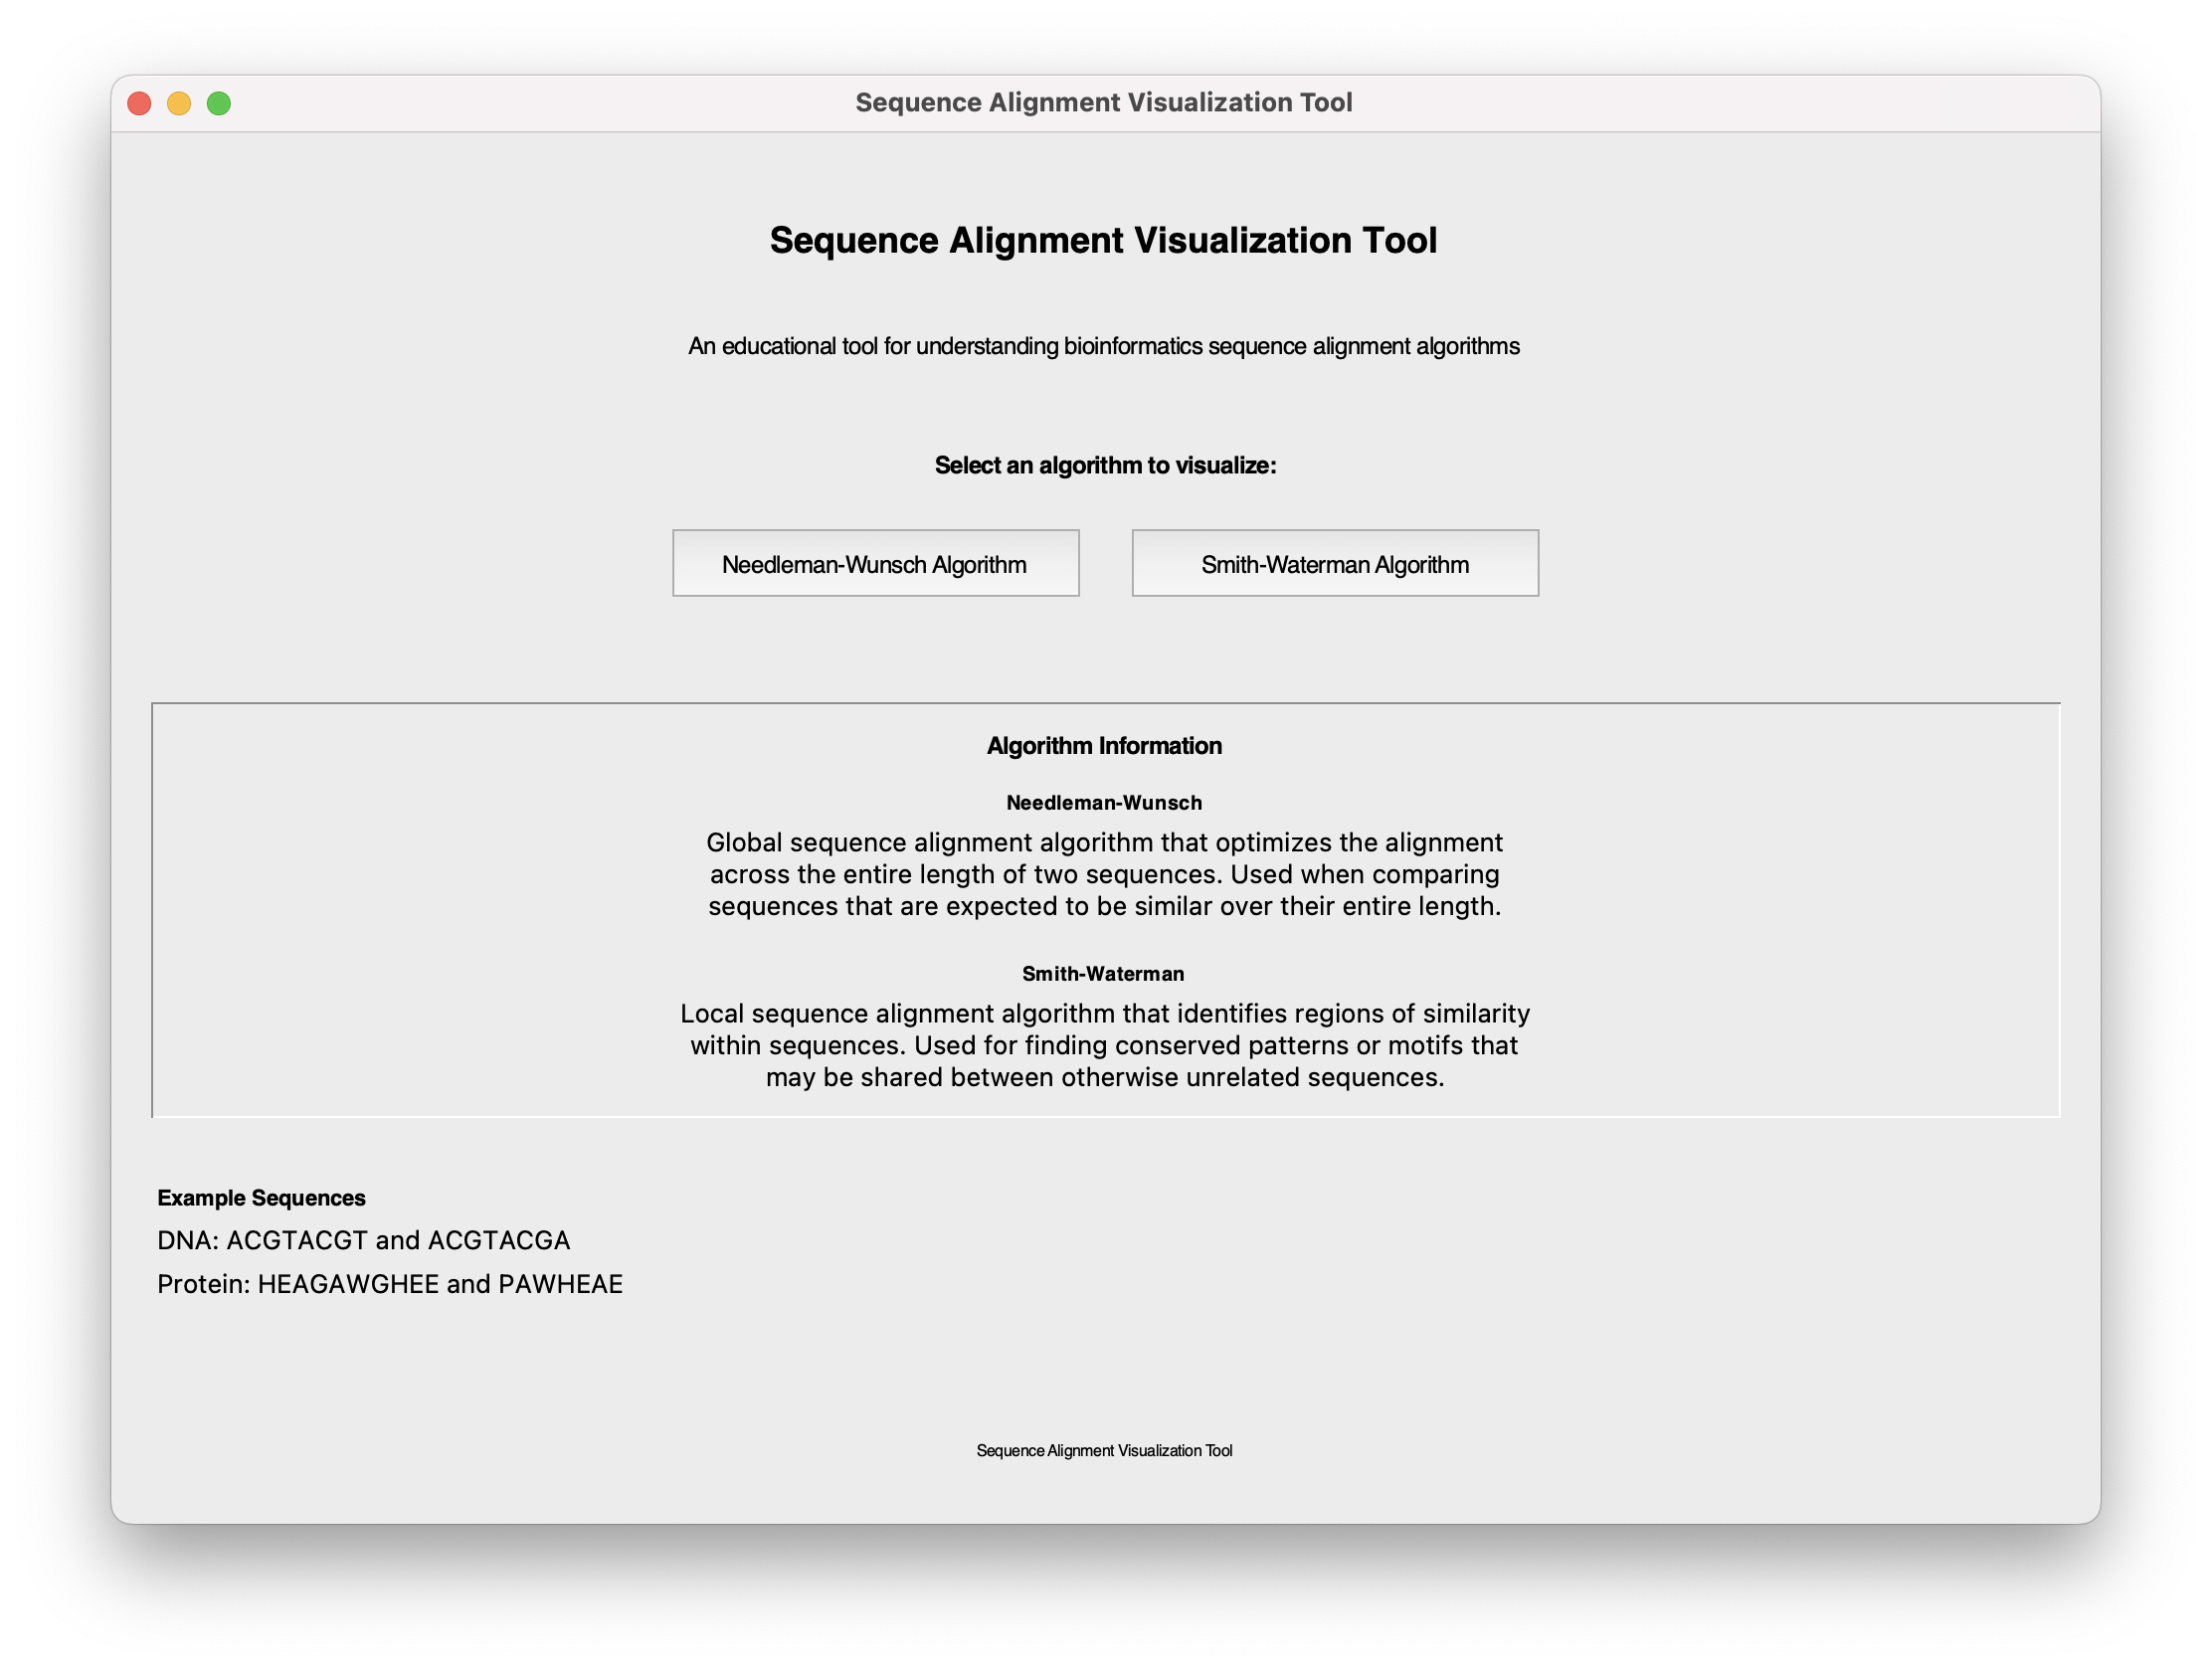
\includegraphics[width=0.7\textwidth]{img/Screenshot 2025-05-06 at 21.15.47.png}
	  \caption{Página de inicio mejorada de la aplicación}
	\end{figure}
	
	\begin{figure}[H]
		\centering
		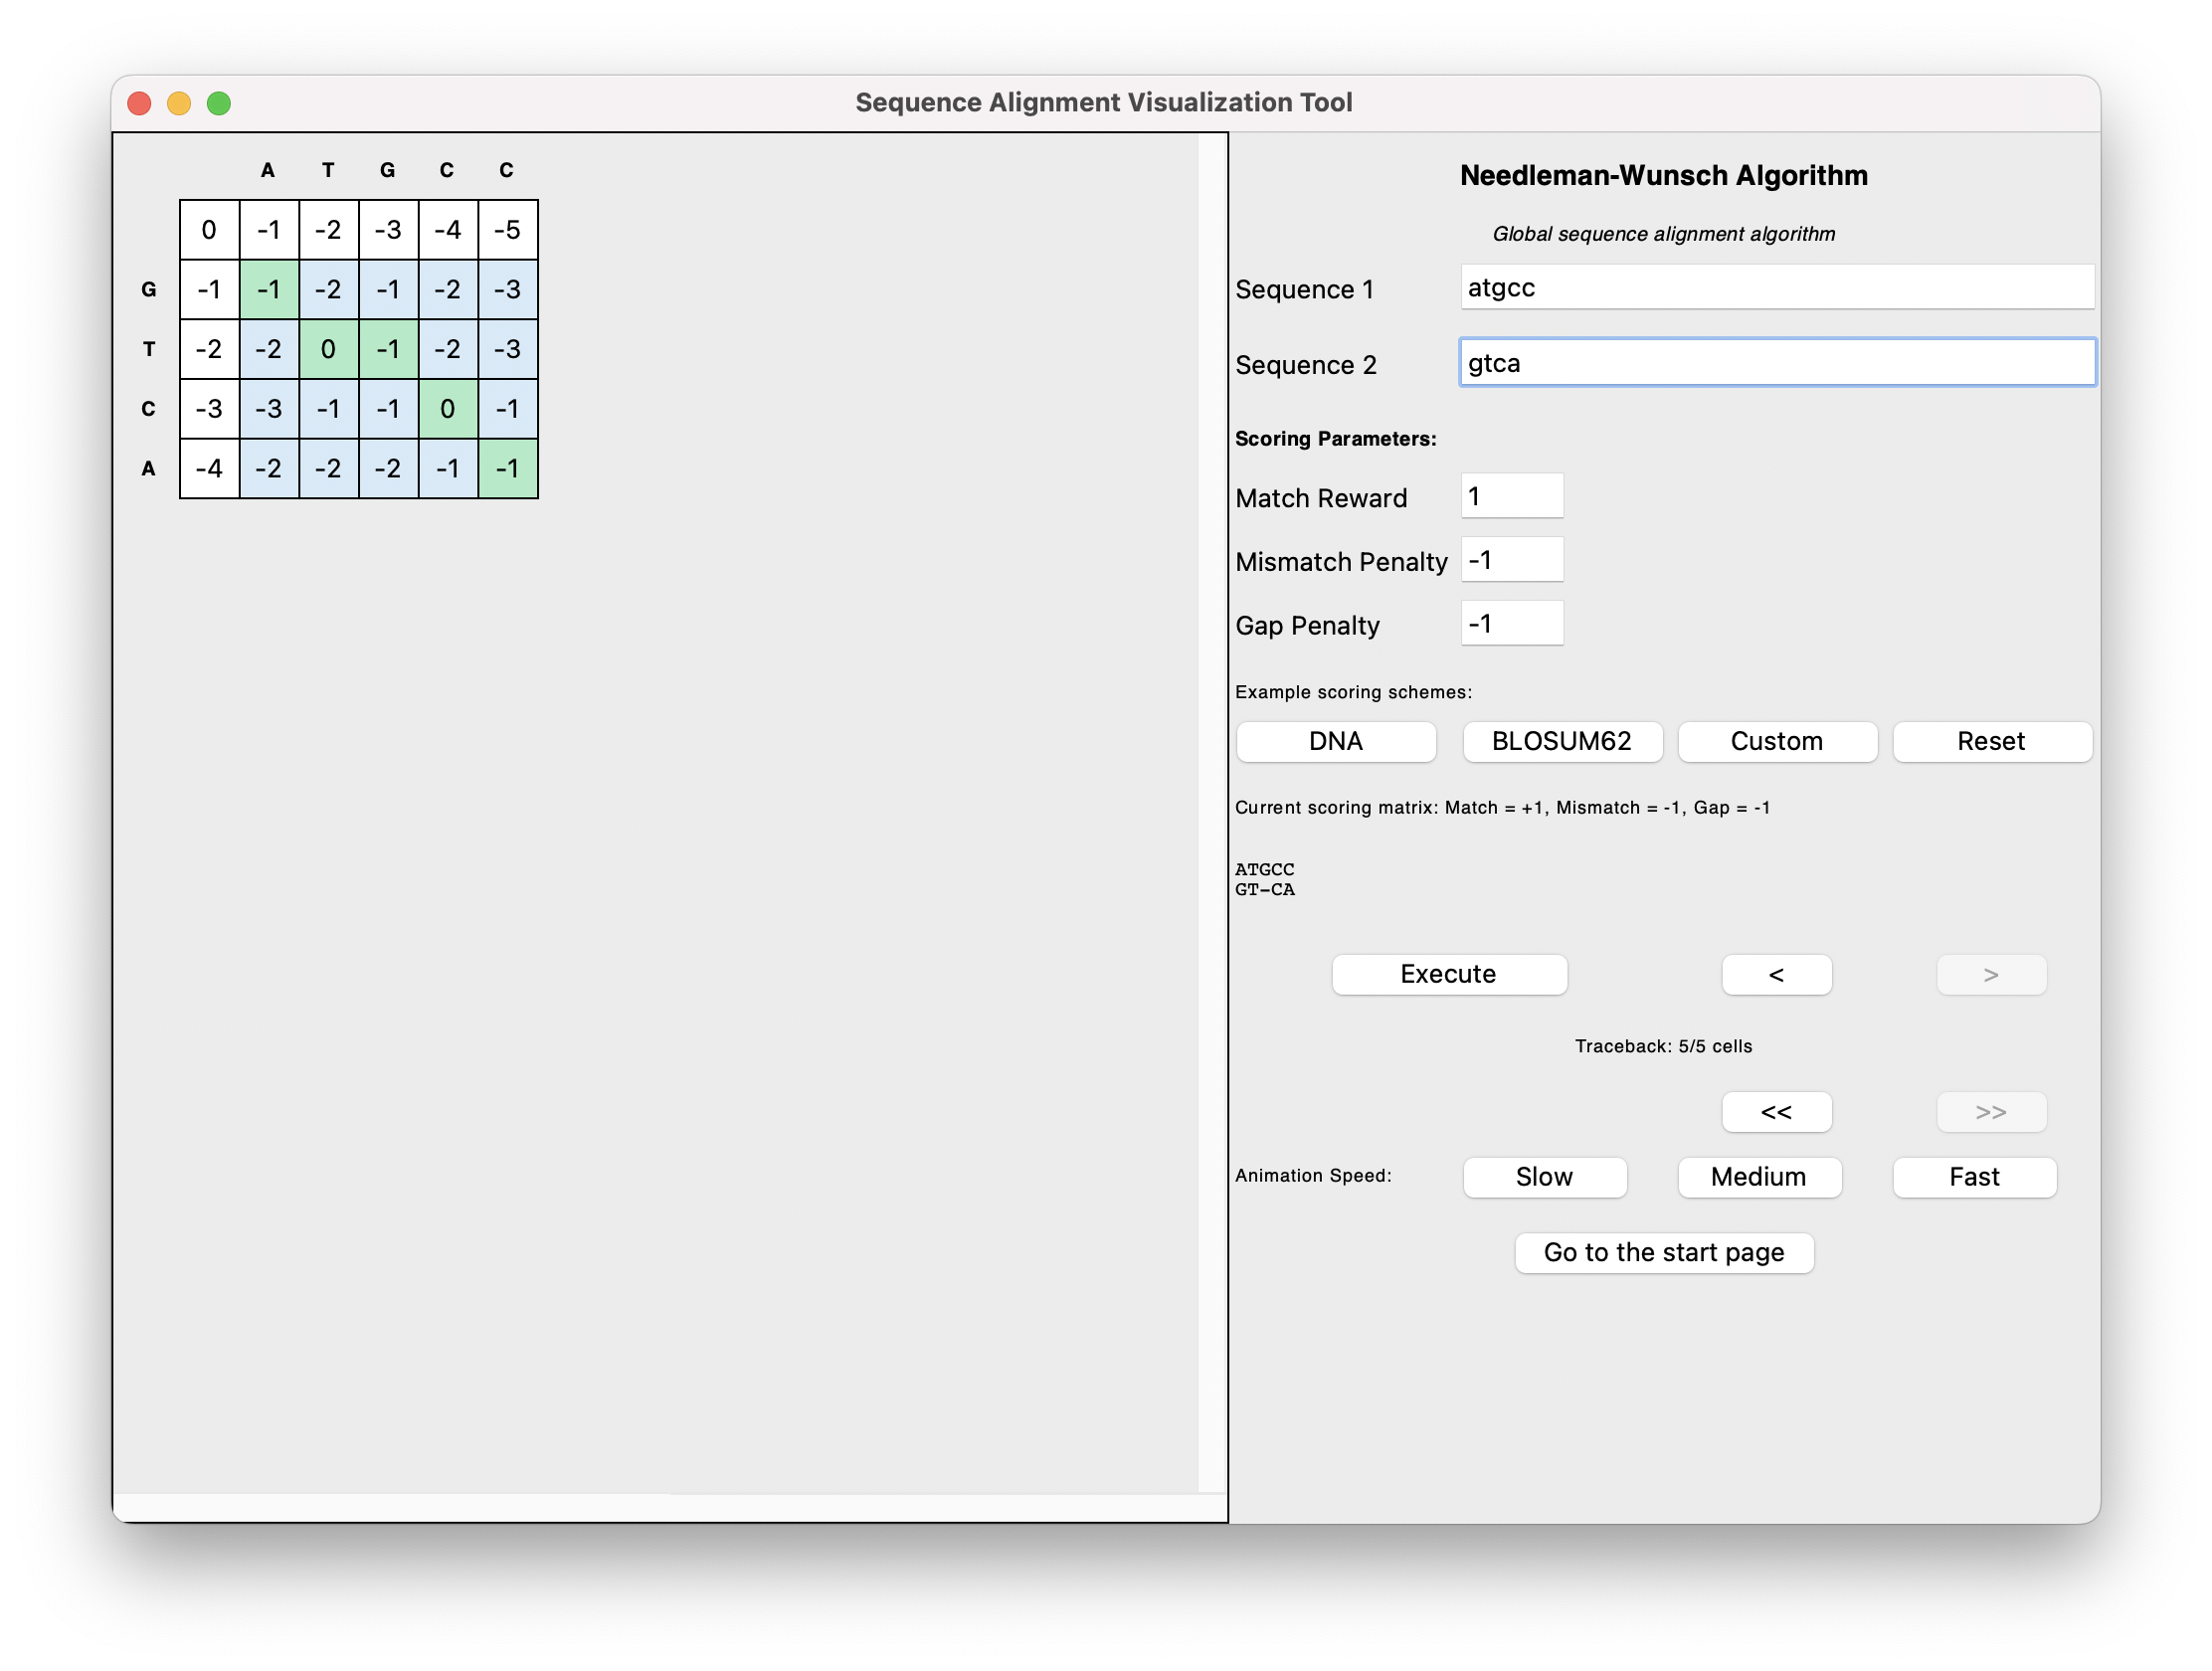
\includegraphics[width=0.7\textwidth]{img/Screenshot 2025-05-06 at 21.16.20.png}
		\caption{Interfaz mejorada de la aplicación}
	\end{figure}
	
  
\section*{Aplicación 2: Implementación de Algoritmos en JavaScript como Proyecto de Título de Mario Muñoz}

\subsection*{Mejoras Propuestas}
\begin{itemize}[noitemsep,topsep=0pt,leftmargin=*]
	\item \textbf{Exportación de resultados}: Añadir funcionalidad para exportar la visualización del alineamiento como imagen y en formato texto, permitiendo a los usuarios guardar o compartir los resultados para su posterior análisis o inclusión en documentos académicos.
	
	\item \textbf{Llenado y recorrido automático}: Implementar una funcionalidad de recorrido automático para el llenado de la matriz y trazado hacia atrás. Actualmente ambos procedimientos deben ser ejecutados de manera manual.
\end{itemize}

\begin{figure}[H]
	\centering
	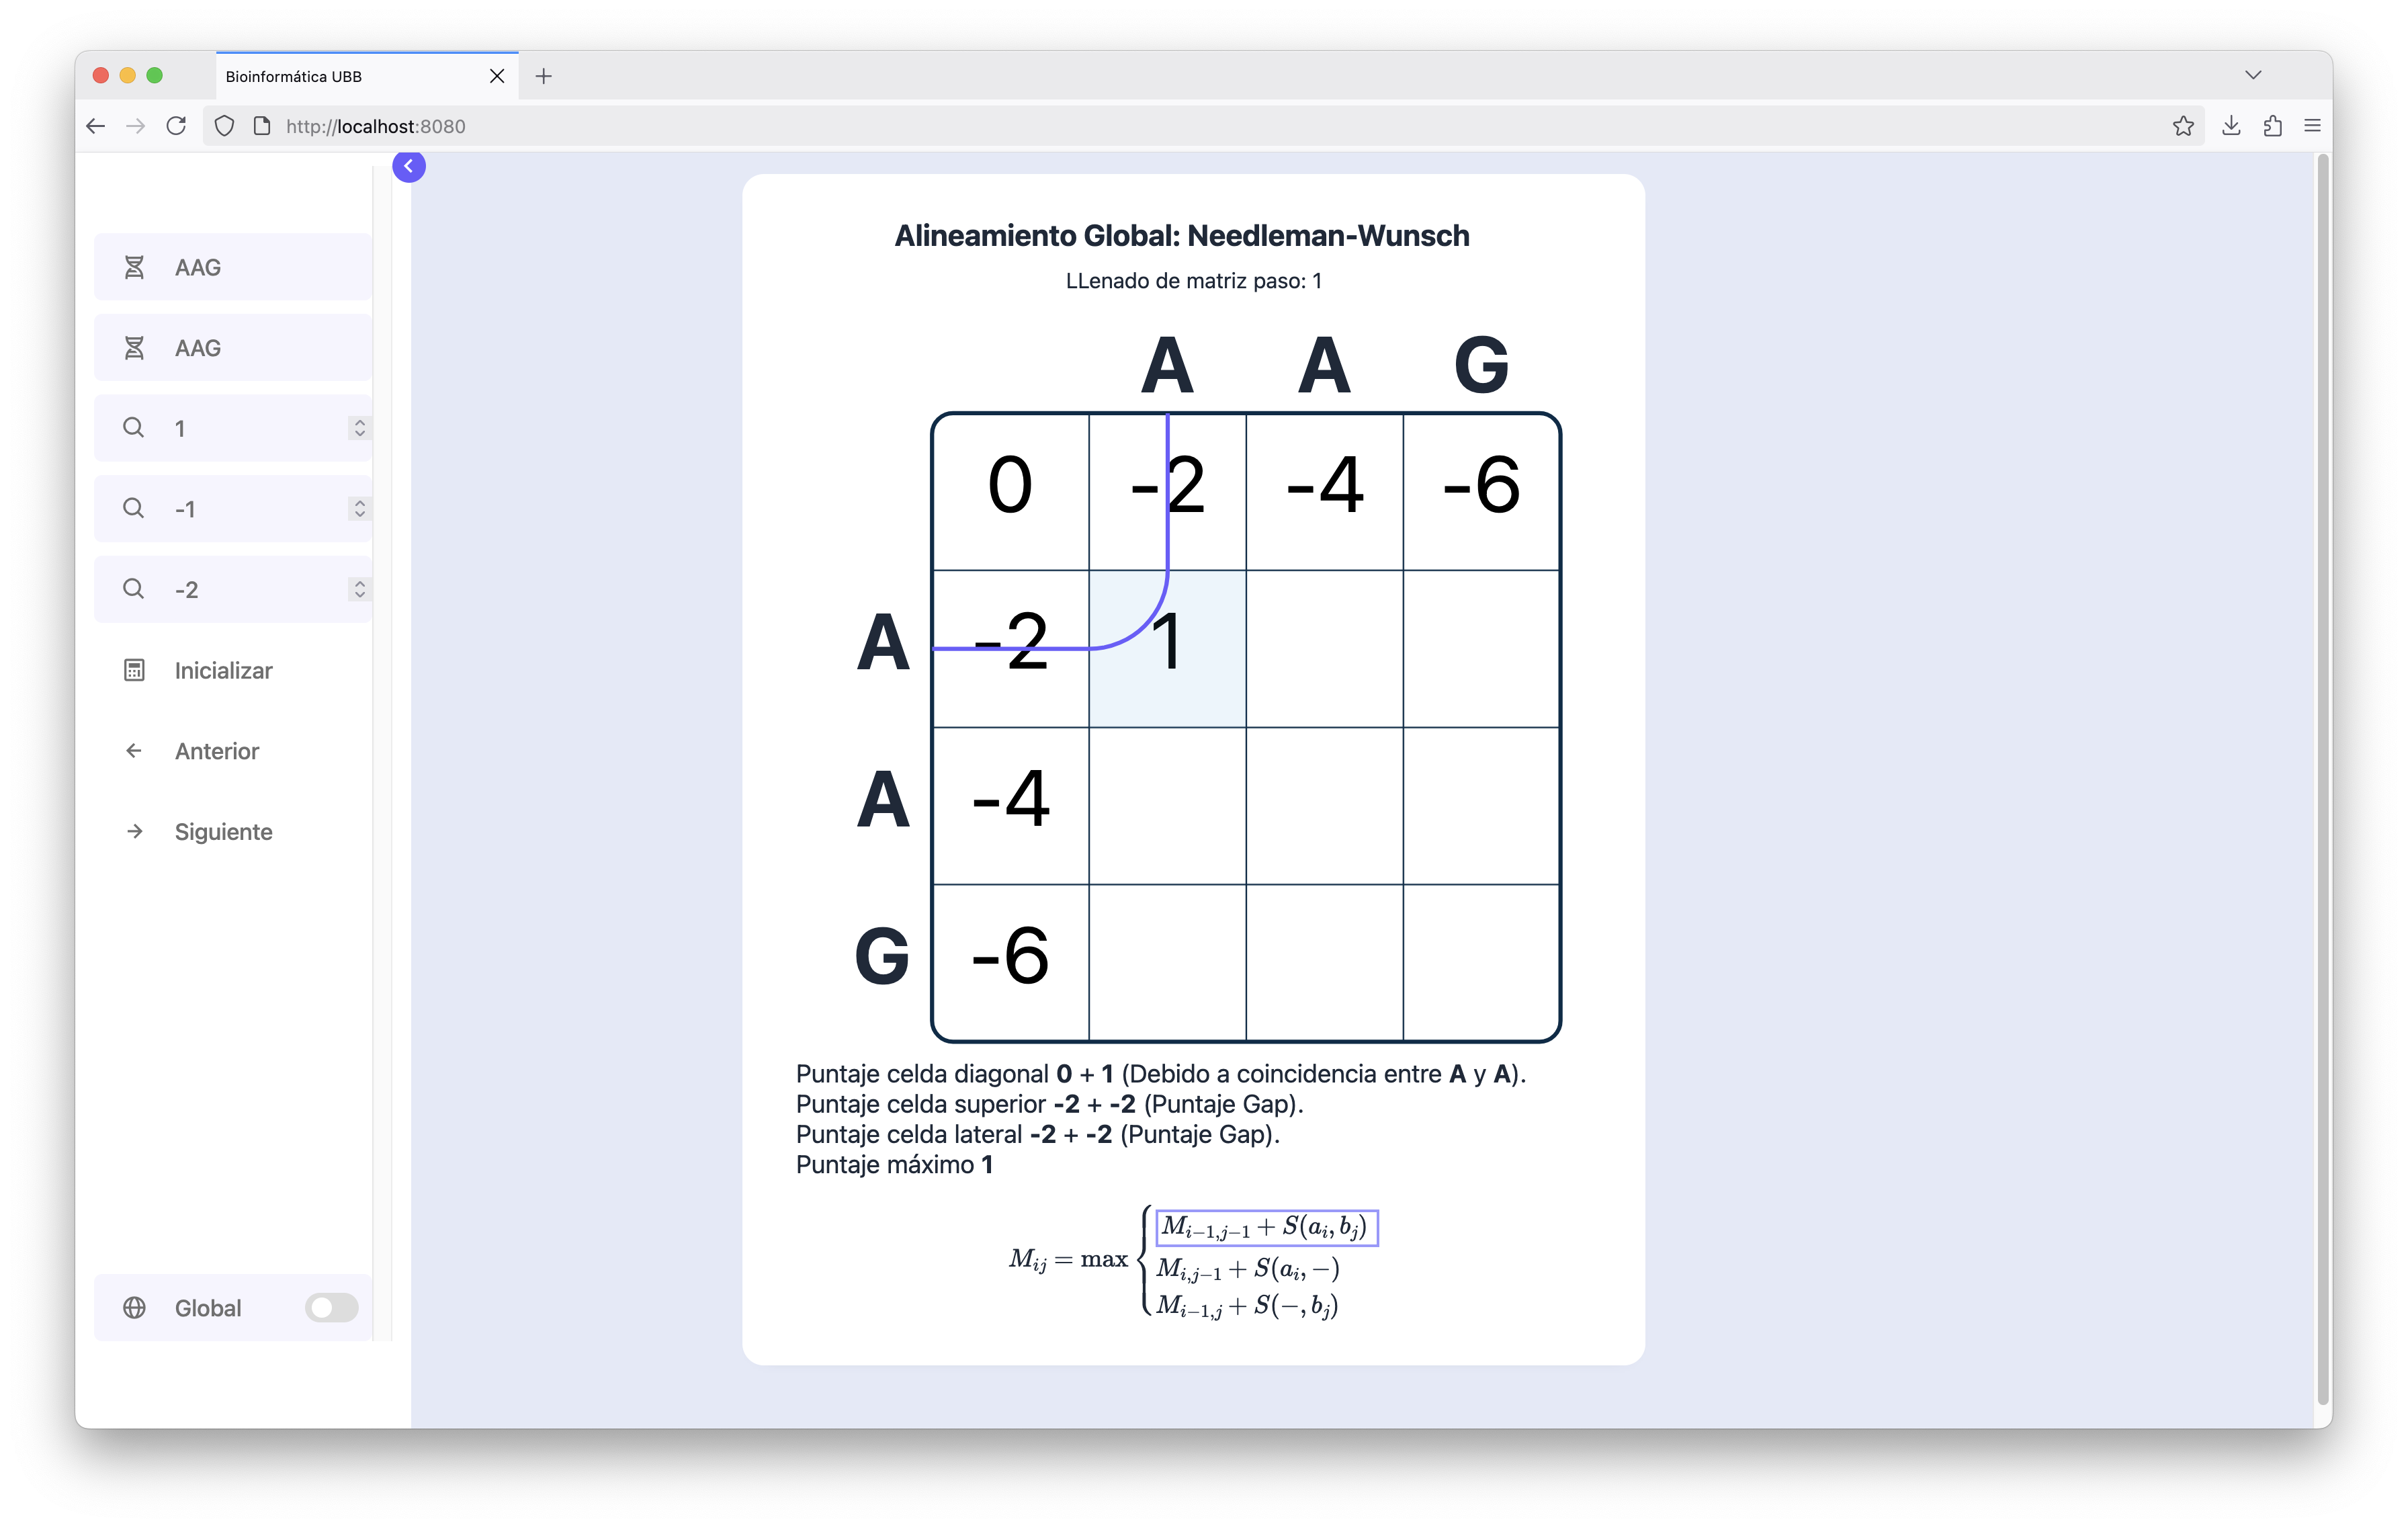
\includegraphics[width=0.7\textwidth]{img/Screenshot 2025-05-06 at 23.51.51.png}
	\caption{Aplicación de Mario Muñoz en entorno local}
\end{figure}

\end{document}